\chapter{المحاليل المنظِّمة ومخططات الغلبة}\label{ch:g12:buffers-predominance}

يذكر تحليل الدم قيمة \omterm{def:g9:acids-bases-ph:ph}{pH} الدم الشرياني: وهي عادةً بين 7.38
و7.42. فالعضلات العاملة تصبّ أحماضًا في الدم، والرئتان تطردان ثنائي أكسيد
الكربون منه، والغذاء يأتي بأحماض وقواعد؛ ومع ذلك لا تكاد قيمة \omterm{def:g9:acids-bases-ph:ph}{pH}
تتحرك. فزوج من الأنواع الكيميائية، حمض وقاعدته، يمتص هذه الصدمات.
ويبيّن هذا الفصل أي شكل من أشكال المزدوجة يغلب عند قيمة \omterm{def:g9:acids-bases-ph:ph}{pH} معيّنة، وكيف تكشف
بضع قطرات من مزدوجة ملوّنة قيمة \omterm{def:g9:acids-bases-ph:ph}{pH}، وكيف يحفظ \omterm{def:g6:pure-substances-and-mixtures:mixture}{خليط} من
حمض وقاعدته قيمة \omterm{def:g9:acids-bases-ph:ph}{pH} ثابتة.

\begin{recall}
المزدوجات حمض/قاعدة، و$K_a$ و$pK_a$؛ \omterm{def:g9:acids-bases-ph:ph}{وpH} \omterm{def:g2:mixing-and-dissolving:dissolve}{المحلول}
(\cref{ch:g12:ka-and-pka}، \cref{ch:g9:acids-bases-ph}).
\end{recall}

\begin{omfigure}
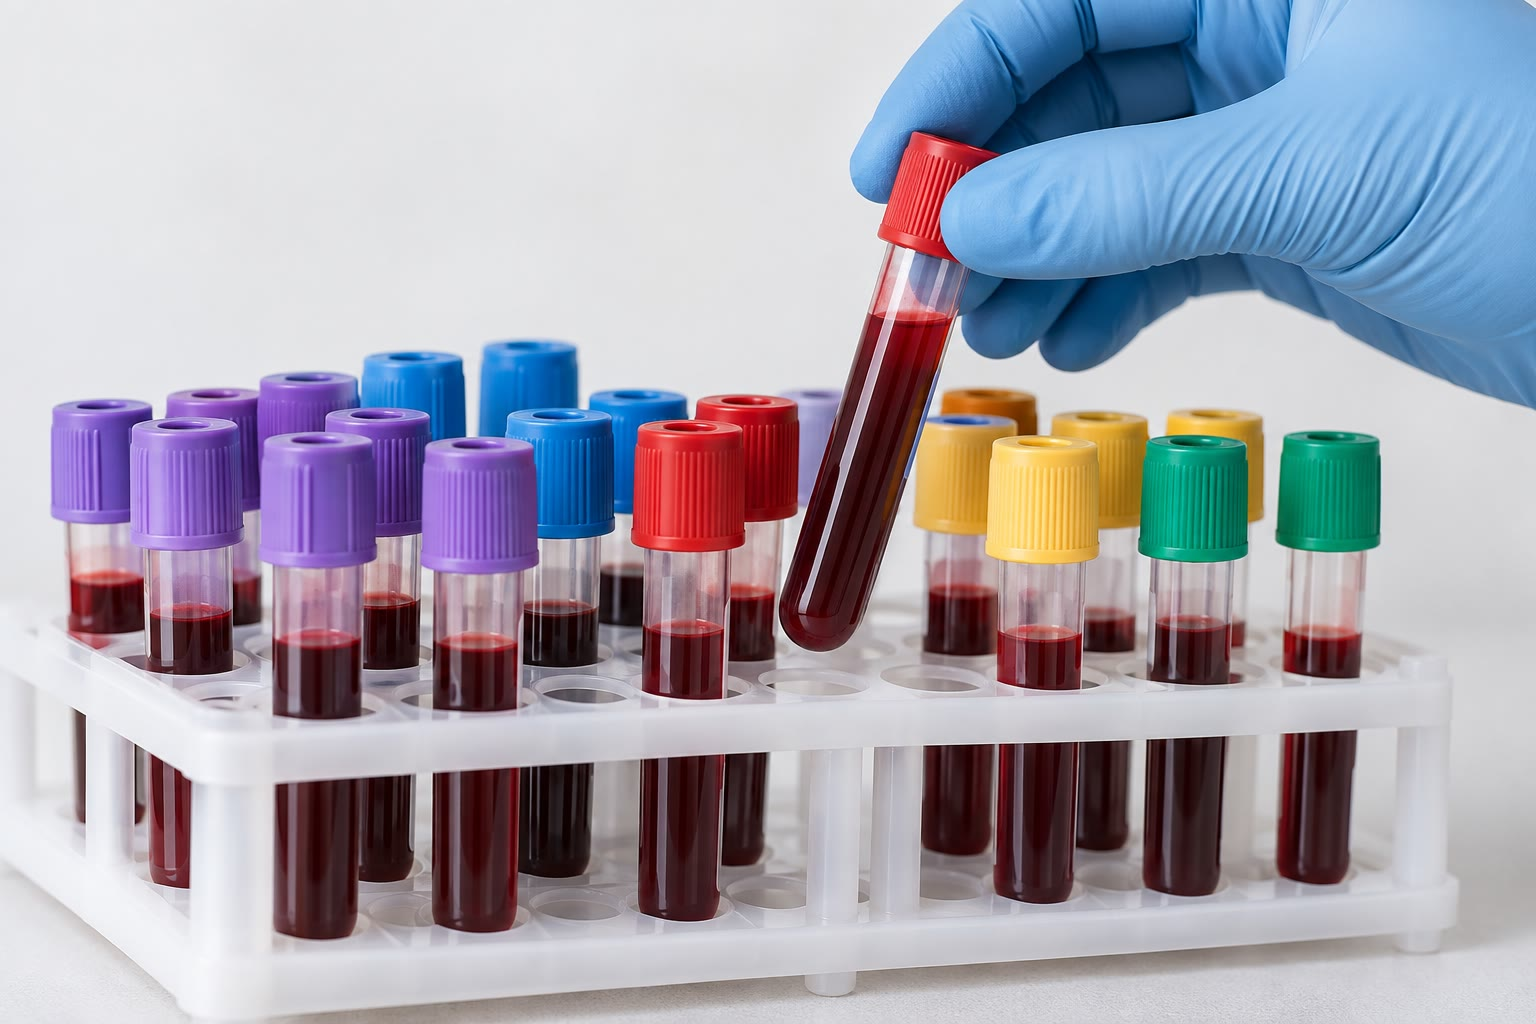
\includegraphics[width=0.45\linewidth]{images/book1/ai/g12-blood-tubes.jpg}

{\small عيّنات دم: قيمة \omterm{def:g9:acids-bases-ph:ph}{pH} فيها محفوظة داخل مجال ضيق.}
\end{omfigure}

\section{مخططات الغلبة}

\begin{proposition}[علاقة هندرسون]\label{prop:g12:buffers-predominance:henderson}
في كل \omterm{def:g6:solutions-and-solubility:solute}{محلول مائي} يحوي المزدوجة $\ce{HA}/\ce{A-}$،
\[
  \mathrm{pH} = pK_a + \log\frac{[\ce{A-}]}{[\ce{HA}]} .
\]
\end{proposition}

\begin{proof}
انطلاقًا من $K_a = \dfrac{[\ce{A-}][\ce{H3O+}]}{[\ce{HA}]c^\circ}$، نأخذ $-\log$
للطرفين: $pK_a = \mathrm{pH} - \log\dfrac{[\ce{A-}]}{[\ce{HA}]}$.
\end{proof}

\begin{definition}[مخطط الغلبة ومخطط التوزيع]\label{def:g12:buffers-predominance:predominance}
\emph{مخطط الغلبة}\index{مخطط الغلبة} لمزدوجة
محور \omterm{def:g9:acids-bases-ph:ph}{pH} مقسوم عند $pK_a$: فتحتها يغلب الحمض HA
($[\ce{HA}] > [\ce{A-}]$)، وفوقها تغلب القاعدة \ce{A-}. و\emph{مخطط
التوزيع}\index{مخطط التوزيع} يبيّن نسبة كل شكل،
$[\ce{HA}]/c$ و$[\ce{A-}]/c$، بدلالة \omterm{def:g9:acids-bases-ph:ph}{pH}؛ ويتقاطع المنحنيان عند
$\mathrm{pH} = pK_a$.
\end{definition}

\begin{method}[رسم مخطط الغلبة]\label{met:g12:buffers-predominance:diagram}
\begin{enumerate}
  \item ارسم محور \omterm{def:g9:acids-bases-ph:ph}{pH} من 0 إلى 14 وعيّن عليه $pK_a$ المزدوجة.
  \item اكتب الحمض على يسار $pK_a$ والقاعدة على يمينها.
  \item \omterm{def:g6:pure-substances-and-mixtures:species}{لنوع كيميائي} له عدة مزدوجات (حمض يعطي ذرتي
        هيدروجين، أو حمض أميني)، عيّن كل قيم $pK_a$: فكل مجال يعود إلى
        شكل واحد.
  \item على بُعد وحدة واحدة من $pK_a$، تكون النسبة قد بلغت 10 إلى 1: فيكون الشكل
        الثانوي دون \qty{10}{\percent}.
\end{enumerate}
\end{method}

\begin{omfigure}
\begin{tikzpicture}[font=\small, x=0.62cm]
  % ledger: pka:ethanoic, pka:methanoic, kb:NH3, ka:H2CO3
  \foreach \y/\pk/\acid/\base in {0/3.74/{\ce{HCOOH}}/{\ce{HCOO-}},
      -1.0/4.76/{\ce{CH3COOH}}/{\ce{CH3COO-}}, -2.0/6.37/{\ce{CO2,H2O}}/{\ce{HCO3-}},
      -3.0/9.26/{\ce{NH4+}}/{\ce{NH3}}} {
    \fill[omThm!20] (0,\y) rectangle (\pk,\y+0.5);
    \fill[omDef!20] (\pk,\y) rectangle (14,\y+0.5);
    \draw[black!50] (0,\y) rectangle (14,\y+0.5);
    \node at (\pk/2,\y+0.25) {\acid};
    \node at ({(\pk+14)/2},\y+0.25) {\base};
    \draw[thick] (\pk,\y-0.08) -- (\pk,\y+0.58);
    \node[font=\scriptsize, anchor=south] at (\pk,\y+0.55) {\pk};
  }
  \draw[->] (0,-3.4) -- (14.5,-3.4) node[right] {pH};
  \foreach \k in {0,2,4,6,8,10,12,14} \draw (\k,-3.35) -- (\k,-3.45) node[below, font=\scriptsize] {\k};
\end{tikzpicture}

{\small مخططات الغلبة لأربع مزدوجات: يغلب الحمض (على اليسار، بالأحمر)
تحت قيمة $pK_a$ له، وتغلب القاعدة (على اليمين، بالأزرق) فوقها.}
\end{omfigure}

\begin{omfigure}
\begin{minipage}{0.49\linewidth}
\begin{tikzpicture}
\begin{axis}[width=\linewidth, height=5cm, xmin=0, xmax=14, ymin=0, ymax=1.05,
    xlabel={\babelsublr{pH}}, ylabel={النسبة}, axis lines*=left, ymajorgrids,
    grid style={gray!20}, tick label style={font=\scriptsize},
    label style={font=\small}, title={\small حمض الإيثانويك},
    title style={yshift=-4pt}]
  \addplot[very thick, omThm] table[x=pH, y=HA] {figdata/out/grade-12-buffers-predominance-a.dat};
  \addplot[very thick, omDef] table[x=pH, y=A] {figdata/out/grade-12-buffers-predominance-a.dat};
  \addplot[dashed, black!50] coordinates {(4.76,0) (4.76,1)};
  \node[font=\scriptsize, omThm] at (axis cs:2.2,0.85) {\ce{CH3COOH}};
  \node[font=\scriptsize, omDef] at (axis cs:7.6,0.85) {\ce{CH3COO-}};
\end{axis}
\end{tikzpicture}
\end{minipage}\hfill
\begin{minipage}{0.49\linewidth}
\begin{tikzpicture}
\begin{axis}[width=\linewidth, height=5cm, xmin=0, xmax=14, ymin=0, ymax=1.05,
    xlabel={\babelsublr{pH}}, ylabel={النسبة}, axis lines*=left, ymajorgrids,
    grid style={gray!20}, tick label style={font=\scriptsize},
    label style={font=\small}, title={\small الغليسين},
    title style={yshift=-4pt}]
  \addplot[very thick, omThm] table[x=pH, y=cation] {figdata/out/grade-12-buffers-predominance-b.dat};
  \addplot[very thick, omMeth] table[x=pH, y=zwitterion] {figdata/out/grade-12-buffers-predominance-b.dat};
  \addplot[very thick, omDef] table[x=pH, y=anion] {figdata/out/grade-12-buffers-predominance-b.dat};
  \node[font=\scriptsize, omThm] at (axis cs:1.0,0.55) {كاتيون};
  \node[font=\scriptsize, omMeth] at (axis cs:6.1,0.88) {أيون مزدوج};
  \node[font=\scriptsize, omDef] at (axis cs:12.6,0.55) {أنيون};
\end{axis}
\end{tikzpicture}
\end{minipage}

{\small مخططات التوزيع، محسوبة من قيم $pK_a$. يسارًا:
حمض الإيثانويك، ويتقاطع المنحنيان عند 4.76. يمينًا: الغليسين،
\ce{H2N-CH2-COOH}، بمزدوجتين (قيمتا $pK_a$ هما 2.35 و9.78): \omterm{def:g9:ions:ion}{الكاتيون}
\ce{H3N+-CH2-COOH}، \omterm{def:g9:ions:ion}{والأيون} المزدوج \ce{H3N+-CH2-COO-} \omterm{def:g9:ions:ion}{والأنيون}
\ce{H2N-CH2-COO-}.}
\end{omfigure}

\begin{example}[الغليسين في الجسم]\label{ex:g12:buffers-predominance:glycine}
% ledger: pka:glycine1, pka:glycine2, ph:blood
عند قيمة \omterm{def:g9:acids-bases-ph:ph}{pH} الدم، نحو 7.4، يقع الغليسين بين قيمتي $pK_a$
له: فيكون كله تقريبًا على هيئة \omterm{def:g9:ions:ion}{أيون} مزدوج، يحمل
شحنة موجبة على نيتروجينه وشحنة سالبة على مجموعة الكربوكسيلات،
وهو متعادل في مجمله. وكل حمض أميني يسلك السلوك نفسه.
\end{example}

\section{الكواشف الملوّنة}


\begin{definition}[الكاشف الملوّن، مجال تغيّر اللون]\label{def:g12:buffers-predominance:indicator}
\emph{الكاشف الملوّن}\index{كاشف ملوّن} \omterm{def:g12:ka-and-pka:bronsted}{مزدوجة حمض/قاعدة}
$\ce{HInd}/\ce{Ind-}$ لشكليها لونان مختلفان، تُستعمل بكميات صغيرة
جدًا. و\emph{مجال تغيّر لونه}\index{مجال تغيّر اللون}
هو مجال قيم \omterm{def:g9:acids-bases-ph:ph}{pH} الذي يُرى فيه اللون يتغير، أي تقريبًا من
$pK_a - 1$ إلى $pK_a + 1$: فتحته يُرى لون \ce{HInd}، وفوقه
لون \ce{Ind-}، وبينهما مزيج من اللونين.
\end{definition}

\begin{omfigure}
\begin{tikzpicture}[font=\small, x=0.62cm]
  % ledger: ind:methyl-red, ind:BBT, ind:phenolphthalein, ind:thymol-blue, ind:range-rule
  \foreach \y/\name/\a/\b/\ca/\cm/\cb in {
      0/{أحمر الميثيل}/4.2/6.3/red!70/orange/yellow!80,
      -0.8/{أزرق البروموثيمول}/6.0/7.6/yellow!80/green!60/blue!60,
      -1.6/{الفينول فثالين}/8.0/10.0/white/magenta!25/magenta!70} {
    \fill[\ca] (0,\y) rectangle (\a,\y+0.5);
    \shade[left color=\ca, right color=\cb] (\a,\y) rectangle (\b,\y+0.5);
    \fill[\cb] (\b,\y) rectangle (14,\y+0.5);
    \draw[black!50] (0,\y) rectangle (14,\y+0.5);
    \node[anchor=east] at (-0.2,\y+0.25) {\name};
  }
  \fill[red!65] (0,-2.4) rectangle (1.2,-1.9);
  \shade[left color=red!65, right color=yellow!80] (1.2,-2.4) rectangle (2.8,-1.9);
  \fill[yellow!80] (2.8,-2.4) rectangle (8.0,-1.9);
  \shade[left color=yellow!80, right color=blue!60] (8.0,-2.4) rectangle (9.1,-1.9);
  \fill[blue!60] (9.1,-2.4) rectangle (14,-1.9);
  \draw[black!50] (0,-2.4) rectangle (14,-1.9);
  \node[anchor=east] at (-0.2,-2.15) {أزرق الثيمول};
  \draw[->] (0,-2.8) -- (14.5,-2.8) node[right] {pH};
  \foreach \k in {0,2,4,6,8,10,12,14} \draw (\k,-2.75) -- (\k,-2.85) node[below, font=\scriptsize] {\k};
\end{tikzpicture}

{\small ألوان أربعة كواشف بدلالة \omterm{def:g9:acids-bases-ph:ph}{pH}؛ والأجزاء المظللة هي
مجالات تغيّر اللون. ولأزرق الثيمول، بمزدوجتيه، مجالا
تغيّر.}
\end{omfigure}

\begin{method}[اختيار كاشف ملوّن]\label{met:g12:buffers-predominance:indicator}
لكشف اللحظة التي يتجاوز فيها \omterm{def:g2:mixing-and-dissolving:dissolve}{محلول} قيمة \omterm{def:g9:acids-bases-ph:ph}{pH} معيّنة (قيمة \omterm{def:g9:acids-bases-ph:ph}{pH} في نهاية
\omterm{def:g11:titration:titration}{معايرة}، مثلًا)، اختر كاشفًا يحوي \omterm{def:g12:buffers-predominance:indicator}{مجال تغيّر لونه}
تلك القيمة: فيتغير اللون عندها بالضبط.
\end{method}

\section{المحاليل المنظِّمة}

\begin{definition}[المحلول المنظِّم]\label{def:g12:buffers-predominance:buffer}
\emph{المحلول المنظِّم}\index{محلول منظم} \omterm{def:g2:mixing-and-dissolving:dissolve}{محلول} لا تكاد قيمة \omterm{def:g9:acids-bases-ph:ph}{pH} فيه
تتغير حين يضاف إليه قليل من حمض أو قاعدة، أو حين
يُخفَّف. ويتكوّن عادةً من \omterm{def:g12:ka-and-pka:strong-acid}{حمض ضعيف} وقاعدته المرافقة بكميات
متقاربة؛ فتكون قيمة \omterm{def:g9:acids-bases-ph:ph}{pH} فيه عندئذ قريبة من $pK_a$ المزدوجة.
\end{definition}

\begin{proposition}[لماذا يقاوم المحلول المنظِّم]\label{prop:g12:buffers-predominance:buffer}
في \omterm{def:g2:mixing-and-dissolving:dissolve}{محلول} منظِّم من \ce{HA} و\ce{A-}، يستهلك \ce{A-} الحمضَ القوي المضاف
(\ce{A- + H3O+ -> HA + H2O}) ويستهلك \ce{HA} القاعدةَ القوية المضافة
(\ce{HA + OH- -> A- + H2O})؛ فلا تتغير النسبة $[\ce{A-}]/[\ce{HA}]$، ومن ثم
قيمة \omterm{def:g9:acids-bases-ph:ph}{pH}، إلا قليلًا. \omterm{def:g10:concentration-and-dilution:dilution}{والتخفيف} لا يغيّر النسبة إطلاقًا.
\end{proposition}

\begin{proof}
بحسب علاقة هندرسون لا تتوقف قيمة \omterm{def:g9:acids-bases-ph:ph}{pH} إلا على النسبة. فإضافة
\qty{1}{mmol} من حمض إلى \omterm{def:g2:mixing-and-dissolving:dissolve}{محلول} منظِّم يحوي \qty{10}{mmol} من كل شكل
تغيّر النسبة من $10/10$ إلى $9/11$، وتغيّر قيمة \omterm{def:g9:acids-bases-ph:ph}{pH} بمقدار
$\log(9/11) = -0.09$ فقط.
\end{proof}

\begin{omfigure}
\begin{tikzpicture}
\begin{axis}[width=0.75\linewidth, height=5.6cm, xmin=0, xmax=10, ymin=0,
    ymax=8, xlabel={\foreignlanguage{arabic}{\ce{HCl} المضاف بتركيز \qty{0.10}{mol/L} \babelsublr{(\si{mL})}}},
    ylabel={\babelsublr{pH}}, axis lines*=left, ymajorgrids, grid style={gray!20},
    tick label style={font=\small}, label style={font=\small},
    legend style={font=\small, at={(0.98,0.97)}, anchor=north east,
    draw=none, fill=white}, legend cell align=left]
  % ledger: pka:ethanoic (buffer recipe: exercise data)
  \addplot[very thick, omThm, mark=*, mark size=1.3pt] table[x=V, y=water]
    {figdata/out/grade-12-buffers-predominance-c.dat};
  \addplot[very thick, omDef, mark=*, mark size=1.3pt] table[x=V, y=buffer]
    {figdata/out/grade-12-buffers-predominance-c.dat};
  \legend{{\foreignlanguage{arabic}{\qty{100}{mL} من الماء النقي}}, {\foreignlanguage{arabic}{\qty{100}{mL} من محلول الإيثانوات المنظِّم}}}
\end{axis}
\end{tikzpicture}

{\small إضافة حمض الهيدروكلوريك إلى الماء النقي وإلى \omterm{def:g2:mixing-and-dissolving:dissolve}{محلول} منظِّم من
حمض الإيثانويك وإيثانوات الصوديوم (\qty{0.10}{mol/L} لكل منهما). فتنخفض قيمة \omterm{def:g9:acids-bases-ph:ph}{pH}
الماء من 7 إلى نحو 2؛ وقيمة \omterm{def:g9:acids-bases-ph:ph}{pH} \omterm{def:g12:buffers-predominance:buffer}{المحلول المنظِّم} من 4.76 إلى 4.67.}
\end{omfigure}

\begin{method}[تحضير محلول منظِّم]\label{met:g12:buffers-predominance:prepare}
\begin{enumerate}
  \item اختر مزدوجة تقع قيمة $pK_a$ لها على بُعد وحدة واحدة على الأكثر من قيمة \omterm{def:g9:acids-bases-ph:ph}{pH} المطلوبة
        (ويُفضَّل أن تكون قريبة منها).
  \item احسب النسبة $[\ce{A-}]/[\ce{HA}] = 10^{\mathrm{pH} - pK_a}$.
  \item اخلط \omterm{def:g12:ka-and-pka:strong-acid}{الحمض الضعيف} وملحًا لقاعدته بهذه النسبة، بتراكيز
        مرتفعة بما يكفي لامتصاص كميات الحمض أو القاعدة
        المضافة.
\end{enumerate}
\end{method}

\begin{inthelab}[تحضير محلول منظِّم قيمة pH فيه 4.8]
يُخلط \qty{50.0}{mL} من حمض الإيثانويك بتركيز \qty{0.10}{mol/L} مع
\qty{50.0}{mL} من إيثانوات الصوديوم بتركيز \qty{0.10}{mol/L}؛ فيقرأ \omterm{def:g9:acids-bases-ph:ph-paper}{مقياس pH}
نحو 4.8. وبضع قطرات من حمض الهيدروكلوريك بتركيز \qty{1}{mol/L} لا تكاد تحرك
القراءة، بينما تخفضها القطرات نفسها في \qty{100}{mL} من الماء المقطر
إلى نحو 3.
\end{inthelab}

\section{المحاليل المنظِّمة في الكائنات الحية}

\begin{example}[المحلول المنظِّم في الدم]\label{ex:g12:buffers-predominance:blood}
% ledger: pk:blood-bicarb, ph:blood, hco3:blood
\omterm{def:g12:buffers-predominance:buffer}{المحلول المنظِّم} الرئيسي في الدم هو مزدوجة ثنائي أكسيد الكربون \omterm{def:g6:solutions-and-solubility:solute}{المذاب}
\omterm{def:g9:ions:ion}{وأيون} الهيدروجينوكربونات، $\ce{CO2,H2O}/\ce{HCO3-}$. وفي الدم، يستعمل
علماء وظائف الأعضاء لها العلاقة $\mathrm{pH} = 6.1 +
\log\big([\ce{HCO3-}]/[\ce{CO2}]\big)$. فالرئتان تزيلان ثنائي أكسيد الكربون،
والكليتان تضبطان الهيدروجينوكربونات: فتحفظان معًا النسبة،
ومن ثم قيمة \omterm{def:g9:acids-bases-ph:ph}{pH}.
\end{example}

\begin{omfigure}
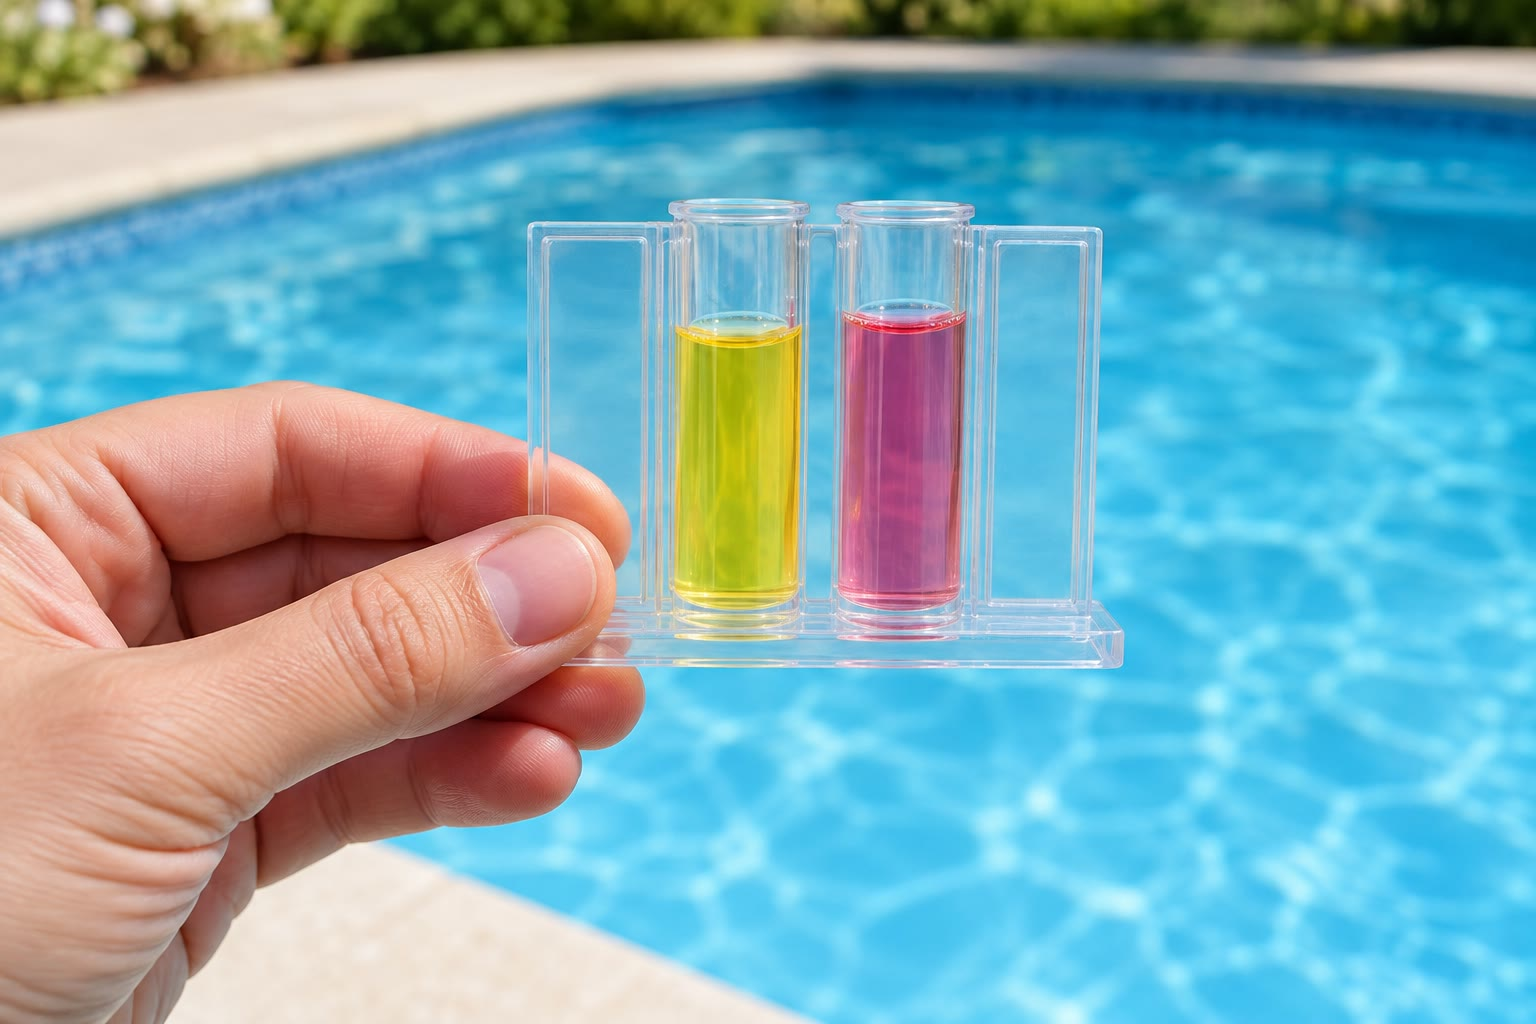
\includegraphics[width=0.45\linewidth]{images/book1/ai/g12-pool-test.jpg}

{\small اختبار ماء المسبح: ألوان الكواشف تعطي قيمة
\omterm{def:g9:acids-bases-ph:ph}{pH}.}
\end{omfigure}

\section{تمارين}


\begin{exercise}[$\star$]\label{exo:g12:buffers-predominance:1}
أي شكلي المزدوجة $\ce{CH3COOH}/\ce{CH3COO-}$ ($pK_a = 4.76$)
يغلب عند \omterm{def:g9:acids-bases-ph:ph}{pH} 2، وعند \omterm{def:g9:acids-bases-ph:ph}{pH} 4.76 وعند \omterm{def:g9:acids-bases-ph:ph}{pH} 7؟
\end{exercise}

\begin{exercise}[$\star$]\label{exo:g12:buffers-predominance:2}
على مخطط توزيع حمض الإيثانويك، اقرأ نسبة
\ce{CH3COO-} عند \omterm{def:g9:acids-bases-ph:ph}{pH} 4 وعند \omterm{def:g9:acids-bases-ph:ph}{pH} 6.
\end{exercise}

\begin{exercise}[$\star$]\label{exo:g12:buffers-predominance:3}
أي لون يُظهر أزرق البروموثيمول عند \omterm{def:g9:acids-bases-ph:ph}{pH} 5؟ وعند \omterm{def:g9:acids-bases-ph:ph}{pH} 7؟ وعند \omterm{def:g9:acids-bases-ph:ph}{pH} 9؟
\end{exercise}

\begin{exercise}[$\star$]\label{exo:g12:buffers-predominance:4}
أي شكلي المزدوجة $\ce{NH4+}/\ce{NH3}$ يغلب في \omterm{def:g2:mixing-and-dissolving:dissolve}{محلول} عند
\omterm{def:g9:acids-bases-ph:ph}{pH} 7.4؟ وعند \omterm{def:g9:acids-bases-ph:ph}{pH} 11؟
\end{exercise}

\begin{exercise}[$\star$]\label{exo:g12:buffers-predominance:5}
لماذا تُستعمل الكواشف الملوّنة بكميات صغيرة جدًا؟
\end{exercise}

\begin{exercise}[$\star\star$]\label{exo:g12:buffers-predominance:6}
احسب النسبة $[\ce{CH3COO-}]/[\ce{CH3COOH}]$ عند \omterm{def:g9:acids-bases-ph:ph}{pH} 3.76 و4.76
و5.76.
\end{exercise}

\begin{exercise}[$\star\star$]\label{exo:g12:buffers-predominance:7}
تنتهي \omterm{def:g11:titration:titration}{معايرة} عند \omterm{def:g9:acids-bases-ph:ph}{pH} 8.7. أي الكواشف الأربعة في الشكل
تختار؟ ولماذا لا تختار أحمر الميثيل؟
\end{exercise}

\begin{exercise}[$\star\star$]\label{exo:g12:buffers-predominance:8}
يحوي \omterm{def:g2:mixing-and-dissolving:dissolve}{محلول} منظِّم \qty{0.20}{mol/L} من حمض الإيثانويك
و\qty{0.10}{mol/L} من إيثانوات الصوديوم. احسب قيمة \omterm{def:g9:acids-bases-ph:ph}{pH} فيه.
\end{exercise}

\begin{exercise}[$\star\star$]\label{exo:g12:buffers-predominance:9}
مستعينًا بمخطط الغليسين، أعطِ الشكل الغالب عند \omterm{def:g9:acids-bases-ph:ph}{pH} 1 و6 و12،
مع شحنته.
\end{exercise}

\begin{exercise}[$\star\star$]\label{exo:g12:buffers-predominance:10}
اقرأ منحنيي الاستجابة: بكم تنخفض قيمة \omterm{def:g9:acids-bases-ph:ph}{pH} الماء بعد
إضافة \qty{1.0}{mL} من الحمض؟ وقيمة \omterm{def:g9:acids-bases-ph:ph}{pH} \omterm{def:g12:buffers-predominance:buffer}{المحلول المنظِّم}؟
\end{exercise}

\begin{exercise}[$\star\star$]\label{exo:g12:buffers-predominance:11}
أي مزدوجة من مزدوجات شكل الغلبة تختار لتحضير
\omterm{def:g2:mixing-and-dissolving:dissolve}{محلول} منظِّم قيمة \omterm{def:g9:acids-bases-ph:ph}{pH} فيه 9.5؟ وبأي نسبة تخلط شكليها؟
\end{exercise}

\begin{exercise}[$\star\star\star$]\label{exo:g12:buffers-predominance:12}
يتلقى \omterm{def:g2:mixing-and-dissolving:dissolve}{محلول} الإيثانوات المنظِّم في الشكل (\qty{10}{mmol} من كل شكل)
حمض الهيدروكلوريك. فما كمية الحمض التي يستطيع تلقيها قبل أن تنخفض قيمة \omterm{def:g9:acids-bases-ph:ph}{pH} فيه
بوحدة واحدة؟ ولماذا يُقال إن \omterm{def:g2:mixing-and-dissolving:dissolve}{للمحلول} المنظِّم الأشد تركيزًا
سعةً أكبر؟
\end{exercise}

\begin{exercise}[$\star\star\star$]\label{exo:g12:buffers-predominance:13}
ما حجم \omterm{def:g2:mixing-and-dissolving:dissolve}{محلول} إيثانوات الصوديوم بتركيز \qty{0.10}{mol/L} الذي يجب
إضافته إلى \qty{100}{mL} من حمض الإيثانويك بتركيز \qty{0.10}{mol/L} للحصول على
\omterm{def:g2:mixing-and-dissolving:dissolve}{محلول} منظِّم قيمة \omterm{def:g9:acids-bases-ph:ph}{pH} فيه 5.0؟
\end{exercise}

\begin{exercise}[$\star\star\star$]\label{exo:g12:buffers-predominance:14}
لأزرق الثيمول مجالا تغيّر للون. اشرح السبب، وأعطِ
لونه عند \omterm{def:g9:acids-bases-ph:ph}{pH} 1 و5 و10.
\end{exercise}

\begin{exercise}[$\star\star\star$]\label{exo:g12:buffers-predominance:15}
يُخفَّف \omterm{def:g2:mixing-and-dissolving:dissolve}{محلول} منظِّم قيمة \omterm{def:g9:acids-bases-ph:ph}{pH} فيه 4.76 عشر مرات بالماء المقطر. فما
قيمة \omterm{def:g9:acids-bases-ph:ph}{pH} الجديدة، بحسب علاقة هندرسون؟ وماذا يحدث إذا خُفّف \omterm{def:g12:ka-and-pka:strong-acid}{حمض
قوي} له قيمة \omterm{def:g9:acids-bases-ph:ph}{pH} نفسها عشر مرات؟
\end{exercise}

\section{مسألة: المحلول المنظِّم في الدم}

\begin{problem}[{مسألة نهاية الأسبوع --- ما النسبة بين الهيدروجينوكربونات
وثنائي أكسيد الكربون التي تحفظ قيمة pH الدم عند 7.4؟}]
\label{pb:g12:buffers-predominance:1}
% ledger: pk:blood-bicarb, ph:blood, hco3:blood
قيمة \omterm{def:g9:acids-bases-ph:ph}{pH} الدم الشرياني عادةً بين 7.38 و7.42. ومحلوله المنظِّم
الرئيسي هو المزدوجة $\ce{CO2,H2O}/\ce{HCO3-}$، التي يستعمل لها علماء وظائف الأعضاء
العلاقة $\mathrm{pH} = 6.1 + \log\big([\ce{HCO3-}]/[\ce{CO2}]\big)$. والتركيز
العادي للهيدروجينوكربونات في الدم من 22 إلى \qty{28}{mmol/L}.

\medskip
\noindent\textbf{الجزء الأول --- المزدوجة.}
\begin{enumerate}
  \item اكتب تفاعل ثنائي أكسيد الكربون \omterm{def:g6:solutions-and-solubility:solute}{المذاب} مع الماء الذي
        يعطي \omterm{def:g9:ions:ion}{أيونات} الهيدروجينوكربونات.
  \item أي النوعين هو الحمض، وأيهما القاعدة؟
  \item تختلف القيمة 6.1 عن القيمة 6.37 في جدول $pK_a$. أعطِ
        سببًا لذلك (فكّر في درجة حرارة الجسم وفي \omterm{def:g9:ions:ion}{الأيونات}
        الأخرى الموجودة).
  \item ما كمية الهيدروجينوكربونات في \qty{5.0}{L} من الدم
        بتركيز \qty{24}{mmol/L}؟
\end{enumerate}

\medskip
\noindent\textbf{الجزء الثاني --- الغلبة.}
\begin{enumerate}[resume]
  \item ارسم \omterm{def:g12:buffers-predominance:predominance}{مخطط الغلبة} للمزدوجة مع $pK = 6.1$.
  \item أي الشكلين يغلب في الدم؟
  \item أالدم حمضي قليلًا أم قاعدي قليلًا؟
\end{enumerate}

\medskip
\noindent\textbf{الجزء الثالث --- النسبة.}
\begin{enumerate}[resume]
  \item احسب، مستعينًا بالعلاقة، النسبة $[\ce{HCO3-}]/[\ce{CO2}]$
        عند \omterm{def:g9:acids-bases-ph:ph}{pH} 7.4.
  \item مع $[\ce{HCO3-}] = \qty{24}{mmol/L}$، احسب $[\ce{CO2}]$.
  \item احسب النسبة عند طرفي المجال العادي، 7.38
        و7.42.
  \item ما نسبة المزدوجة الموجودة على هيئة هيدروجينوكربونات
        عند \omterm{def:g9:acids-bases-ph:ph}{pH} 7.4؟
  \item قد يبلغ الدم المفرط القاعدية \omterm{def:g9:acids-bases-ph:ph}{pH} 7.6. فما النسبة
        عندئذ؟
\end{enumerate}

\medskip
\noindent\textbf{الجزء الرابع --- حين يختل التوازن.}
\begin{enumerate}[resume]
  \item خلال جهد شديد، تدخل الأحماض الدم. فأي شكلي
        المزدوجة يستهلكها؟ اكتب التفاعل.
  \item لو انخفضت قيمة \omterm{def:g9:acids-bases-ph:ph}{pH} إلى 7.1، فكم تصير النسبة؟
  \item مع بقاء الهيدروجينوكربونات على حالها، بكم كان يجب أن يزداد ثنائي
        أكسيد الكربون؟ وماذا تفعل الرئتان للمقاومة؟
  \item لماذا يكون \omterm{def:g12:ka-and-pka:strong-acid}{الحمض الضعيف} مع قاعدته، لا \omterm{def:g12:ka-and-pka:strong-acid}{الحمض القوي}، الأداة
        المناسبة لحفظ قيمة \omterm{def:g9:acids-bases-ph:ph}{pH}؟
  \item بكم تتغير قيمة \omterm{def:g9:acids-bases-ph:ph}{pH} إذا قُسم التركيزان كلاهما
        على اثنين؟ ولماذا؟
  \item اذكر الجواب النهائي: ما النسبة بين الهيدروجينوكربونات وثنائي أكسيد
        الكربون في الدم عند \omterm{def:g9:acids-bases-ph:ph}{pH} 7.4؟
\end{enumerate}
\end{problem}
